\chapter[Referencial Teórico]{Referencial Teórico}
\label{ch:referencial}

Neste capítulo são apresentadas as bases teóricas para a elaboração do 
aplicativo com o objetivo de facilitar o entedimento dos termos utilizados. 
O capítulo está estruturado em seções. Na seção 2.2, serão apresentados os 
conceitos sobre o ciclo menstrual feminino e suas fases, e na seção 2.3, serão 
apresentados os fundamentos sobre o Sistema de Recomendação e alguns algoritmos 
utilizados nessa área.

\section{O Ciclo Menstrual}

O ciclo menstrual é um fenômeno biológico 
na qual a característica notável é o fluxo sanguíneo vaginal \cite{guyton2012}.
Ele é cíclico e ocorre como resultado direto de variações das concentrações
hormonais secretadas pelo eixo hipotálamo-hipófise-gonadal. Estudos sugerem
que essas flutuações hormonais, principalmente de estrogênio e progesterona,
que ocorrem no decorrer do ciclo, podem influenciar as emoções,
comportamento e a cognição \cite{poroma2014}, afetando
diretamente no dia-a-dia, como por exemplo, o desempenho nas tarefas
cotidianas ou relacionamentos interpessoais.


O ciclo idealizado tem como base 28 dias. Por convenção, o primeiro dia de
menstruação é a marca do início do ciclo e a marca do final do ciclo
anterior, caso não tenha ocorrido a gravidez \cite{lenton1984a}. O ciclo
pode ser dividido em duas fases, a fase folicular e a fase lútea
\cite{brondin2008}. O período da menstruação está presente no início da
fase folicular e o período da ovulação está situado entre as duas fases.
Mais informações sobre as fases, quanto tempo elas duram, quais hormônios
atuam, e a influência deles nas mulheres, serão pontuadas nas subseções
seguintes.


\subsection{Fase Folicular}

A fase folicular é a primeira fase do ciclo menstrual, começa com o início
da menstruação e termina com a ovulação. Enquanto ocorre a menstruação e os
hormônios estimulantes dos ovários (principalmente FSH) estão em concentração
baixa, a fase é referida como fase folicular inicial \cite{lenton1984a}.

Essa é a fase responsável pelo desenvolvimento de folículos, dos quais um
será selecionado e se transformará em um óvulo (corpos lutem), que dará início
à ovulação. Os folículos desenvolvem-se em resposta ao aumento do hormônio
folículo-estimulante (FSH) (vide Figura \ref{fig01}). Assim que um desses 
folículos for selecionado, o FSH diminui gradativamente, e progressivamente a produção de
estrogênios começará a aumentar. Os estrogénios produzidos pelo folículo em
crescimento são responsáveis também pelo desenvolvimento do endométrio. Essa fase é normalmente 
referida como fase folicular tardia.


Normalmente, mulheres de 18 a 24 anos com ciclo de 28 dias tem a fase com
o comprimento de 14 dias, e mulheres de 40 a 44 anos tem de 10 dias
\cite{lenton1984a}, o que indica a diminuição progressiva do tamanho da
fase folicular com o avanço da idade. Em mulheres jovens, a diferença no
tamanho do ciclo é normalmente provocada por ciclos mais curtos ou mais
longos na fase folicular \cite{lenton1984a}. Ciclos irregulares também
costumam ser pela variação no tamanho da fase folicular, enquanto a fase
lútea segue normalmente com tamanho fixo de 14 dias.


\begin{figure}[h]
	\centering
	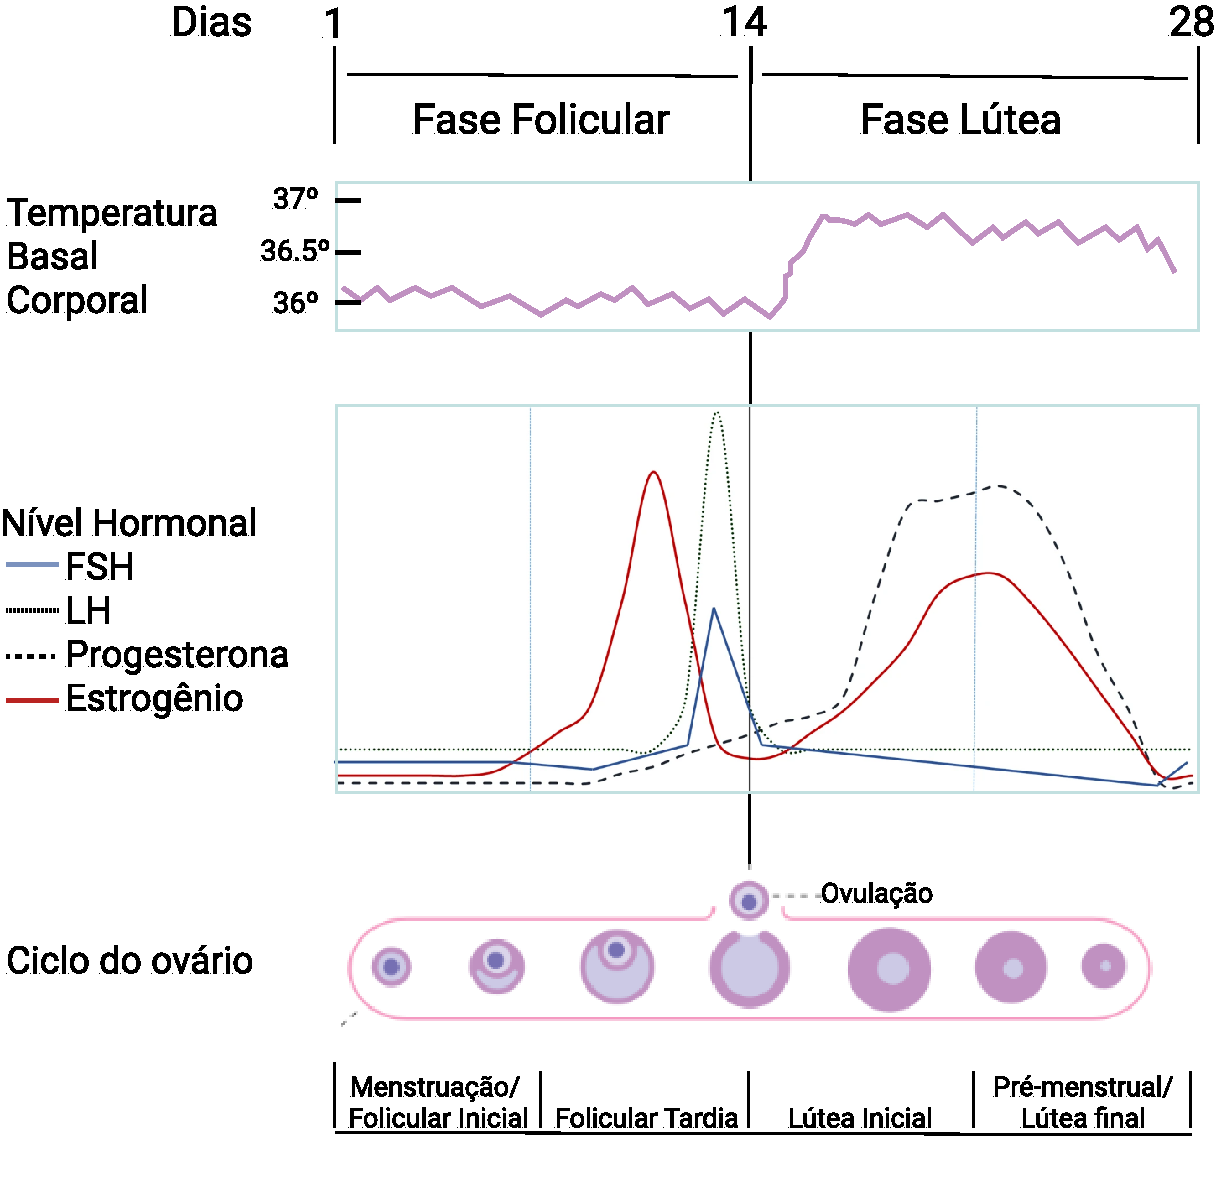
\includegraphics[keepaspectratio=true,scale=0.6]{figuras/ciclomenstrual.pdf}
	\caption{Ciclo Menstrual (Fonte: Elaborado pela Autora, baseado em \cite{draper2018} e \cite{reed2018})}
        \label{fig01}
\end{figure}

Os estudos a seguir demonstraram que no domínio cognitivo 
as funções verbais, espaciais e de memória variam ao longo do ciclo 
menstrual. Na fase folícular, ou quando há baixos níveis de estradiol, 
uma melhora no desempenho em tarefas espaciais foi relatada 
\cite{hausmann2000,maki2002, courvoisier2013, becker1982, phillips1992}, 
e uma melhora nas habilidades verbais foi identificada 
no final da fase folicular quando há altos níveis de estradiol 
\cite{Rosenberg2002}. No aspecto emocional, alguns estudos relacionaram a 
fase com um aumento na habilidade de reconhecimento facial de emoções 
\cite{derntl2013}. Por fim, dois trabalhos concluem que a realização das tarefas verbais é melhor 
ao final das fases folicular e lútea \cite{Rosenberg2002, solis2004}.


\subsubsection{Menstruação}

A menstruação marca o início do ciclo menstrual e o fim do ciclo anterior 
e é caracterizada pelo fluxo sanguíneo vaginal. Ocorre quando não há 
fecundação no ciclo anterior e é composta por sangue e tecido uterino 
derivado da descamação das paredes internas do útero(endométrio). 
Normalmente, dura cerca de 5 dias, mas pode variar \cite{guyton2012}.

O fluxo do sangramento também varia muito, mas costuma ser mais intenso nos 
primeiros dias. O fluxo menstrual pode ser leve, moderado ou intenso. (adicionar referencia)

\subsection{Ovulação}

A ovulação em si não é uma fase propriamente dita, mas quando referida 
como tal carrega o significado de um período estimado em que há a 
possível liberação do óvulo e maior probabilidade de gravidez. 
A fase também é referida como fase fértil e, neste estudo, é dividida em 
outra fase por sua importância.

A ovulação acontece pelo equilíbrio entre vários hormônios. 
Clinicamente é possível determinar o ciclo ovulatório pelo surgimento do 
LH e a secreção de progesterona da fase lútea \cite{fritz2010}. 
Quando o estradiol chega ao pico, passadas 12 a 14 horas, o LH surge. 
Na sequência, de 10 a 12 horas depois, faz com que o ovócito complete a 
sua maturação, rompendo o folículo. O folículo é liberado na cavidade 
abdominal, dirigindo-se à trompa de Falópio \cite{fritz2010}. 
A subida do LH é o que determina o início da fase lútea.

Como através de um aplicativo não é possível medir o aparecimento do LH 
para determinar o fim da fase folicular e o início da ovulação, 
e a ovulação é estimada através de uma janela, então a ovulação e a fase 
folicular acabarão se sobrepondo nesse estudo.

\subsection{Fase Lútea}

Com o evento da ovulação, o folículo transforma-se em um corpo lúteo, e as 
células das paredes do folículo começam a produção de progesterona para 
preparar o endométrio para a chegada do óvulo no caso de concepção. 
O pico da progesterona dá-se normalmente por volta do vigésimo primeiro 
dia do ciclo \cite{nikas2003}. Caso não haja fecundação, a progesterona 
decai progressivamente e causa novamente a menstruação, continuando assim 
o ciclo.

A fase lútea tem duração de 14 dias e costuma ser constante nas mulheres, 
sem grande variação, mesmo que o tamanho do ciclo varie. É comum no final 
da fase lútea o aparecimeno do transtorno disfórico pré-menstrual(TDPM), 
que também ifluência significativamente os aspectos emocionais e 
comportamentais durante as fases do ciclo menstrual. Esse transtorno 
será mais detalhado na seção 2.2.3.1.

Alguns estudos demonstraram que no domínio cognitivo, as funções verbais, 
espaciais e de memória variam ao longo do ciclo menstrual. Na fase lútea, 
uma melhora no desempenho em tarefas verbais e memoriais foi relatada 
\cite{hausmann2000}. No aspecto emocional, existe uma piora na precisão 
do reconhecimento de emoções faciais, principalmente para emoções negativas, 
e existe um aumento na memória emocional, principalmente a recordação de 
itens negativos ou detalhes periféricos. As mulheres tendem a responder 
mais rapidamente a situações tristes e estressantes ou expressões faciais 
tristes. Relatou-se que quando os níveis de progesterona estão altos, as 
mulheres demonstram uma maior tendência a perceber expressões de medo. 
Também há evidências que o cortisol, hormônio do estresse, parece se elevar 
na fase lútea\cite{kirschbaum1999}.

\subsubsection{Tensão Pré Menstrual e o Transtorno Disfórico Pré Menstrual}

Cerca de 90\% das mulheres em idade reprodutiva experienciam algum tipo de 
sintoma pré-menstrual. Uma menor parcela atende aos critérios da tensão 
pré-menstrual (TPM), e cerca de 10\% são diagnosticadas com o transtorno 
disfórico pré menstrual \cite{mishell2005}. Os sintomas pré-menstruais 
são caracterizados com uma lista de sintomas físicos, cognitivos, 
afetivos e comportamentais que ocorrem ciclicamente e aparecem durante a 
fase lútea \cite{obrien2011}, de uma a duas semanas antes da menstruação. 

Os sintomas da TPM variam entre: depressão, irritabilidade, ansiedade, 
explosões de raiva, retraimento social, sensibilidade mamária, 
inchaço abdominal, dores de cabeça e entre outros. Mais de 200 sintomas 
são ligados a essa síndrome. De acordo com o boletim da ACOG, a TPM pode 
ser diagnosticada se um ou mais desses sintomas forem reportados cinco dias 
antes do início da menstruação, durante três ciclos menstruais. Os sintomas 
devem ser registrados por pelo menos dois ciclos; devem passar dentro de 
quatro dias após o início da menstruação, e retornar apenas depois do 12º dia do 
ciclo \cite{ACOG2000}.

Não existe um teste laboratórial específico que pode ser utilizado para 
diagnóstico da síndrome, mas a organização mundial da saúde utiliza o ICD-9 
código 635.4 para caracterizar a TPM e o Transtorno Disfórico Pré Menstrual(TDPM). 
Não existe separação no diagnóstico entre a TPM e a TDPM \cite{biggs2011}.

\subsection{Método Baseado em Calendário}


No método baseado em calendário, uma contagem através do calendário é usada para determinar 
a fase do ciclo. O auto-relato do primeiro dia de menstruação é 
utilizado como ponto inicial do calendário, e as fases são determinadas 
contando-se \lq \lq n\rq \rq \ números de dias para frente ou de trás para 
a frente a partir da data de início prevista para o próximo ciclo \cite{wideman2013}.

O ciclo base utilizado é normalmente o de 28 dias. Para representar eventos
ovulatórios (próximos a altos níveis de estradiol, e antes de um aumento significativo da
progesterona), é contado 10 a 14 dias a partir do início do ciclo ou de 12 a 14 dias a partir do
dia de previsão para o início do próximo ciclo. Entretanto, enquanto os eventos ovulatórios ocorrem
em média entre esses dias, o momento real da ovulação pode variar significativamente
a partir desta janela. O meio da fase lútea, em que os hormônios ficam 
estabilizados, normalmente é contado de 17 a 21 dias do início do ciclo 
ou de 7 a 9 dias a partir do final do ciclo \cite{wideman2013}. 
A Figura \ref{fig02} representa um ciclo de 28 dias.

Para ciclos maiores ou 
menores que 28 dias a ovulação é adiantada ou atrasada pela diferença 
entre o tamanho do ciclo e o ciclo base de 28 dias. Por exemplo, se for 
um ciclo de 32 dias, a ovulação provavelmente ocorrerá entre o 10º e 18º dia 
a partir do início do ciclo.


\begin{figure}[h]
	\centering
	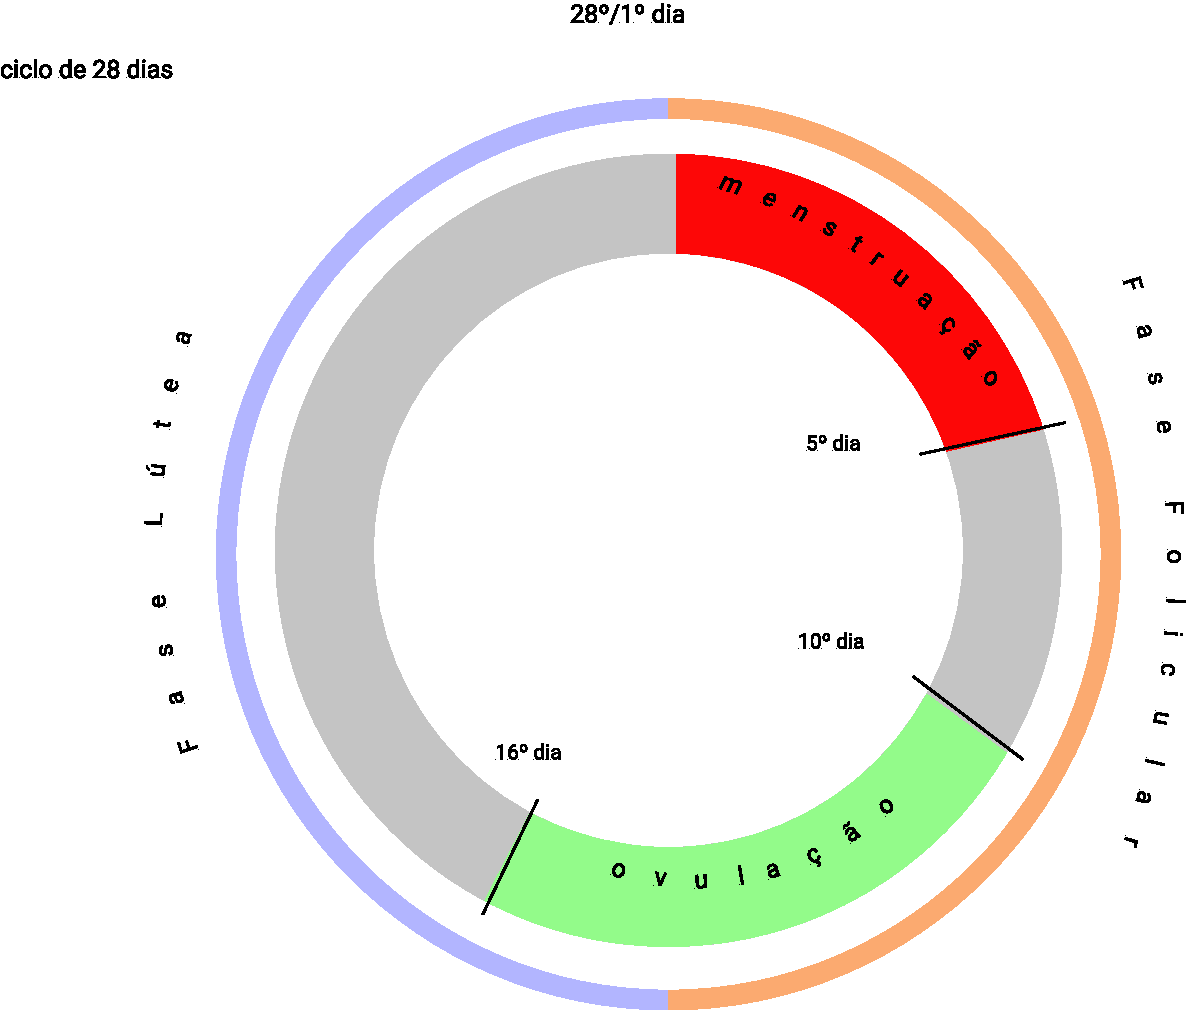
\includegraphics[keepaspectratio=true,scale=0.4]{figuras/Group1.pdf}
	\caption{Calendário do Ciclo Menstrual e suas Fases (Fonte: Elaborado pela Autora.)}
        \label{fig02}
\end{figure}


\section{Sistema de Recomendação}
 
Os sistemas de recomendação (SR) tiveram início em meados dos anos 90 
quando os primeiros trabalhos sobre filtragem colaborativa (FC) 
apareceram \cite{felferning2008} evoluídos pelas academias, 
que continuaram desenvolvendo novas abordagens. 
Ainda é uma área de grande interesse devido à grande quantidade de 
problemas que a envolve e por sua praticidade em lidar com o grande 
número de informações disponível na internet \cite{adomavicius2005}. 
O sistema de recomendação tem como proposta ajudar os usuários a lidarem com esse 
excesso, fornecendo recomendações personalizadas baseadas nas informações 
coletadas, equilibrando fatores como precisão, novidade, dispersão e 
estabilidade\cite{bobadilla2013}.


Os SRs são implementados e possuem literatura 
para áreas de diferentes temas, como música, televisão, livros, 
documentos, \emph{e-learning}, \emph{e-comerce}, aplicações em mercados, 
pesquisa na web e filmes. A maioria dos estudos estão focados 
para recomendação de filmes \cite{bobadilla2013}.
 
Eles coletam informações sobre as preferências 
de seus usuários para um conjunto de itens (livros, filmes, músicas, 
memes, aplicativos, entre outros), e usam de recursos demográficos dos 
usuários (idade, nacionalidade e sexo), informações sociais 
(seguidores, postagens, seguidos), ou informações coletadas através da 
internet das coisas (localização, gps, rfid, sinais de saúde em tempo 
real e outras coisa). Essas informações podem ser adquiridas de maneira 
explícita, por meio de classificações dos usuários, ou implicitamente 
\cite{bobadilla2013}.

De acordo com \citeonline{bobadilla2013}, os sistemas de recomendação 
acompanham a evolução da web. A evolução da web é constituída de três 
fases, a web tradicional, a web social e a internet das coisas. 
Na primeira fase, a geração de sistemas de recomendação usava de 
sites tradicionais para coletar informações de três fonte: dados 
baseados em conteúdo de produtos comprados ou usados; dados 
demográficos coletados nos registros dos usuários, e dados baseados em 
memória, sendo coletados das preferências de itens dos usuários. A segunda 
geração veio com a web 2.0 reunindo informações sociais. A terceira 
geração usa a web 3.0 através de informações fornecidas pelos dispositivos 
integrados na internet(internet das coisas).

Os primeiros sistemas de recomendação focavam em melhorar a precisão da 
recomendação através da filtragem. A maioria dos métodos e algoritmos 
baseados em memória, como por exemplo o KNN, método de agregação, decomposição do valor 
singular, métodos baseados em difusão, entre outros, foram
desenvolvidos e melhorados nesse contexto. Na primeira fase, com a 
abordagem híbrida utilizando a filtragem de conteúdo 
colaborativo-demográfico e colaborativo, ocorreu a melhora na qualidade 
das recomendações. Na segunda fase, algorítimos que incluiam informações 
das redes sociais (ex. algoritmos de
confiança, abordagens sociais adaptativas, análise de redes sociais, 
entre outros) foram adaptados e 
desenvolvidos. Atualmente, os algoritmos híbridos incorporam informações 
de localização em algoritmos de recomendações já existentes \cite{bobadilla2013}. 

Os SRs podem ser, basicamente, classificados em dois grupos: sistemas de recomendação baseados	
em conteúdo e os sistemas de recomendação colaborativos \cite{mauricio}. Os sistemas
de recomendação baseado em conteúdo fazem recomendações baseadas em itens semelhantes
a outros itens já escolhidos pelo usuário e por isso possuem a caracteristica de
diferenciar os interesses do usuário e fazer recomendações mais individualizadas. Já os 
sistemas de recomendação colaborativos fazem recomendações de itens baseado nos interesses 
de outros usuários com perfil semelhante ao do usuário, esses sistemas costumam homogeneizar
os interesses dos usuários, criando grupos com interesses semelhantes. Os algoritmos híbridos 
utilizam das duas abordagens para fazer recomendações.


\subsection{Fundamentos}

De acordo com \citeonline{bobadilla2013}, o processo de geração das recomendações dos SRs é baseado 
na combinação das seguintes considerações:


\begin{itemize}

	\item O tipos de dados disponíveis em seu banco de dados (classificações, informações de registro do usuário, recursos e conteúdo para itens que podem ser
	classificados e relações sociais entre os usuários); 

	\item O algoritmo de filtragem usado (baseado em conteúdo, colaborativo ou híbrido);

	\item O modelo escolhido (baseado em memória ou baseado em modelo);
	
	\item As técnicas empregadas (abordagens probabilísticas, algoritmo de vizinhos mais próximos;
	algoritmos bioinspirados, como redes neurais e genéticas; modelos difusos e entre outros);
	
	\item  Nível de dispersão do banco de dados e escalabilidade desejada;

	\item  Desempenho do sistema (consumo de tempo e memória);

	\item  O objetivo buscado, e

	\item A qualidade desejada dos resultados (novidade, cobertura e
   precisão).

\end{itemize}

Além da classificação pelo tipo de algoritmo de filtragem já citado, os SRs também podem 
ser classificados pelo modelo escolhido \cite{bobadilla2013}: baseado em memória e baseado em modelo. 
Os métodos baseados em memória atuam apenas na matriz de avaliações do usuário para certos itens e utilizam de 
classificações geradas anteriormente para um novo processamento, atualizando sempre os resultados. 
Os métodos baseados em modelo usam as informações pré-existentes para criar um
modelo que gera as recomendações. Esses métodos ficam desatualizado com novas informações do usuário.

A Tabela \ref{tab01} foi adaptada do trabalho de \citeonline{adomavicius2005} e apresenta os algoritmos mais utilizados, 
divididos entre as abordagens de recomendação baseado em conteúdo, colaborativos e híbridos, e nas técnicas 
de recomendação baseadas em heurística e em modelo. 

\begin{table}[]
	\centering
	\caption{Algoritimos Utilizados nas Abordagens de Recomendações}
	\label{tab01}
	\begin{tabular}{|c|c|c|}
	\hline
	\rowcolor[HTML]{C0C0C0} 
	\cellcolor[HTML]{C0C0C0} \textbf{Abordagem} & \multicolumn{2}{c|}{\cellcolor[HTML]{C0C0C0} \textbf{Técnica de Recomendação}} \\ \cline{2-3} 
	\rowcolor[HTML]{C0C0C0} \textbf{de Recomendação}
	\multirow{-2}{*}{\cellcolor[HTML]{C0C0C0}} &  \textbf{Baseada em heurística} & \textbf{Baseada em modelo} \\ \hline
	\textbf{Baseada em Conteúdo	}   & \begin{minipage} [t] {0.3\textwidth} \begin{itemize} \item TF-IDF (recuperação de informação) \item Clustering \end{itemize} \end{minipage} & \begin{minipage} [t] {0.3\textwidth} \begin{itemize} \item Classificador bayesiano \item Clustering \item Árvores de decisão \item Redes Neurais Artificiais \end{itemize} \end{minipage} \\ \hline
	\rowcolor[HTML]{EFEFEF} 
	\textbf{Filtragem Colaborativa}	& \begin{minipage} [t] {0.3\textwidth} \begin{itemize} \item "Vizinhos mais próximos" \item Clustering \item Teoria dos Grafos \end{itemize} \end{minipage} & \begin{minipage} [t] {0.3\textwidth} \begin{itemize} \item  Redes bayesianas \item Clustering \item Redes Neurais Artificiais \item Regressão Linear \item Modelos Probabilísticos \end{itemize} \end{minipage} \\ \hline
	\textbf{Híbrida} &  \begin{minipage} [t] {0.3\textwidth} Combinando conteúdo e componentes colaborativos usando: \begin{itemize} \item Combinação linear de classificações previstas \item Esquemas variados de votação \item incorporação de um componente como parte da heurística para o outro \end{itemize}        \end{minipage} & \begin{minipage} [t] {0.3\textwidth} Combinando conteúdo e componentes colaborativos usando: \begin{itemize} \item incorporação de um componente como parte do modelo para o outro \item construção de um modelo unificado \end{itemize} \end{minipage} \\ \hline
	\end{tabular}
\end{table}

Além das abordagens de recomendação tanto baseadas em conteúdo quanto colaborativas, \citeonline{burke2002} também cita mais três técnicas de recomendação: demográfica, baseada em utilidade e 
baseada em conhecimento. De acordo com \citeonline{burke2002}, os sistemas de recomendação têm: 

\begin{itemize}

	\item \emph{background data}, as informações que o sistema possui antes da recomendação;

	\item dados de entrada, as informações que o usuário deve comunicar ao
	sistema para gerar uma recomendação, e

	\item um algoritmo que combina antecedentes e dados de entrada para chegar às suas sugestões.

\end{itemize}

Na Tabela \ref{tab02}, adaptada do trabalho de \citeonline{burke2002}, os cinco tipos de recomendação tem o sistema de background, entrada e processo brevemente explicados 
assumindo que, \textbf{I} é o conjunto de itens sobre os quais as recomendações são feitas; \textbf{U} é o conjunto de usuários cujas preferências são conhecidas; \textbf{u} 
é o usuário para o qual as recomendações devem ser geradas, e \textbf{i} é algum item para o qual pretende-se prever sua preferência.

\begin{table}[]
	\centering
	\caption{\emph{Background}, Entrada e Processo Utilizados nos Sistemas de Recomendação}
	\label{tab02}
	\begin{tabular}{|c|c|c|c|}
	\hline
	\rowcolor[HTML]{C0C0C0} 
	\textbf{Técnicas} & \textbf{Background} & \textbf{Entrada}  &  \textbf{Processo}  \\ \hline
	\textbf{Colaborativa} & \begin{minipage} [t] {0.2\textwidth} \centering Avaliações de \textbf{U} de itens em \textbf{I}  \end{minipage}  & \begin{minipage} [t] {0.2\textwidth} \centering Avaliações de \textbf{u} dos itens em \textbf{I} \end{minipage}  &  \begin{minipage} [t] {0.2\textwidth}  Identifique usuários em \textbf{U} semelhantes a \textbf{u} e extrapole a partir de suas classificações de \textbf{i}.   \end{minipage}    \\ \hline
	\rowcolor[HTML]{EFEFEF} 
	\textbf{Baseada em Conteúdo} & \begin{minipage} [t] {0.2\textwidth} \centering Características dos itens em \textbf{I}\end{minipage}  & \begin{minipage} [t] {0.2\textwidth} \textbf{u}'s avaliações dos itens em \textbf{I} \end{minipage}  &   \begin{minipage} [t] {0.2\textwidth} Gere um classificador de acordo com \textbf{u}'s comportamento de classificação e use-o em \textbf{i}. \end{minipage} \\ \hline
	\textbf{Demográfica} & \begin{minipage} [t] {0.2\textwidth} \centering Informações demográficas sobre \textbf{U} e suas classificações de itens em \textbf{I}.    \end{minipage}   & \begin{minipage} [t] {0.2\textwidth} Informações demográficas sobre \textbf{u}. \end{minipage}  & \begin{minipage} [t] {0.2\textwidth} Identifique os usuários que são demograficamente semelhantes a \textbf{u} e extrapole a partir de suas classificações de \textbf{i}. \end{minipage}   \\ \hline
	\rowcolor[HTML]{EFEFEF} 
	\textbf{Baseado em utilidade} & \begin{minipage} [t] {0.2\textwidth} \centering Características dos itens em \textbf{I} \end{minipage}  & \begin{minipage} [t] {0.2\textwidth} 
		Uma função de utilidade sobre os itens em \textbf{I} que descreve \textbf{u}'s preferências \end{minipage}   & \begin{minipage} [t] {0.2\textwidth} Aplique a função aos itens e determine a classificação de \textbf{i}.  \end{minipage}  \\ \hline
	\textbf{Baseado em conhecimento}  & \begin{minipage} [t] {0.2\textwidth} \centering Características dos itens em \textbf{I}. Conhecimento de como esses itens atendem às necessidades do usuário.  \end{minipage}  & \begin{minipage} [t] {0.2\textwidth} Uma descrição das necessidades ou interesses de \textbf{u}.\end{minipage}  &  \begin{minipage} [t] {0.2\textwidth}  
		Inferir uma correspondência entre a necessidade de \textbf{i} e \textbf{u}. \end{minipage} \\ \hline
	\end{tabular}
\end{table}



Nas subseções seguintes, serão abordadas alguns dos fundamentos mais específicos dos tipos de filtragens utilizados nos Sistemas de Recomendação.


\subsubsection{Filtragem Baseada em Conteúdo}


Os Sistemas de Recomendação Baseados em Conteúdo fazem recomendações baseadas nas escolhas passadas do usuário \cite{bobadilla2013}. 
Eles realizam consultas e armazenam informações sobre os metadados dos itens que o usuário teve interesse ou não e realizam recomendações 
com base nas informações armazenadas do usuário e de outros itens da base de dados \cite{mauricio}. A partir desta análise, uma semelhança pode ser
estabelecida entre os objetos que um usuário comprou, visitou, ouviu, viu e classificou a outros objetos semelhantes, gerando assim novas recomendações. 

Por exemplo, na recomendação de filmes, o sistema de recomendação baseado em conteúdo 
tenta entender as semelhanças entre os filmes que o usuário classificou e, então, recomenda filmes 
que tenham um alto grau de similaridade nas preferências do usuário (atores, diretores, gênero, assuntos e entre outros) \cite{adomavicius2005}.

Uma das limitações dessa técnica de filtragem é que itens novos não são explorados, só aqueles que são semelhantes 
aos itens já no perfil do usuário, isso leva a uma superespecialização. Em alguns casos, isso pode ser tratado com a 
injeção de aleatóriedade\cite{paulson2003}.


Algumas das técnicas de aprendizado de máquina mais utilizadas incluem: árvore de decisão, \emph{K-means}, redes neurais e classificadores 
bayesiano \cite{son2017}. Por exemplo, o conceito básico do classificador bayesiano visa determinar se um item é preferível examinando informações de 
atributos. Essa técnica é usada para estimar a probabilidade de um item 
pertencer a uma classe $Ci$. A previsão de classificação é calculada usando a 
seguinte função de probabilidade
\begin{equation}
	P(C_{i}|X) = \coprod _{k=1}^{n} P(x_{k}|C_{i})
\end{equation}
onde cada instância de item $X$ é descrita por uma conjunção de valores de atributo de item $x1$, $x2$,… $xk$. 


Esses sistemas de recomendação geralmente necessitam de alguma forma de \emph{feedback} do usuário e isto pode ser 
um problema, pois os usuários tendem a achar essa tarefa tediosa e quanto menos avaliações, mais limitado 
será o conjunto de possíveis recomendações, podendo influenciar negativamente o desempenho \cite{paulson2003}. 

Em técnicas de aprendizado de máquina, o processo de \emph{feedback} é necessário para a aprendizagem e calibração 
do algoritmo e requer constantes atualizações das preferências do usuário, conforme o usuário avalia os itens. Dessa forma, 
as preferências não permanecem estáticas \cite{paulson2003}. 



\subsubsection{Filtragem Colaborativa}

Os Sistemas de Recomendação de Filtragem Colaborativa (FC) dispensam o uso de metadados \cite{mauricio}. 
Em geral, apenas mantêm por quais itens um usuário já demonstrou interesse. O sistema constrói perfis de classificação 
de seus usuários, localiza outros usuários com perfis de classificação 
semelhantes e retorna itens que os usuários semelhantes classificaram 
positivamente \cite{son2017}.

Para prever os votos de usuário a partir de um banco de dados de votos do usuário e de uma amostra ou população de outros usuários, 
\citeonline{breese2013} propôs a seguinte média de votos do usuário, demonstrada na  Eq. \ref{eqn02}, em que a base de dados 
consiste em um conjunto de votos $v_{i,j}$, correspondendo ao voto do usuário $i$ no item $j$. Se $I_{i}$ é o
conjunto de itens nos quais o usuário votou, então pode-se definir o voto médio para o usuário $i$ como:

\begin{equation}
	\label{eqn02}
\overline{v}_{i} = \frac{1}{\left | i \right |} \sum_{j\epsilon I_{i}}^{} v_{i,j}
\end{equation}


Para um sistema particular, a definição do termo \lq\lq semelhante\rq\rq\ é necessária para encontrar 
os \lq\lq vizinhos mais próximos\rq\rq\ do usuário para fazer as recomendações. Este é um dos principais 
pontos onde os sistemas colaborativos diferem. Especificar quais usuários devem ser considerados semelhantes determina o
desempenho do sistema em termos de precisão das recomendações \cite{son2017}.

O algoritmo mais utilizado para FC é o \emph{K Nearest Neighbors} (kNN), ou "vizinhos próximos". O kNN executa 
os três passos seguintes para gerar recomendações: (i) determinar os $k$ vizinhos mais próximos ao usuário; (ii) implementar 
uma abordagem de agregação, com avaliações de itens avaliados pelos vizinhos, mas que não foram avaliados pelo usuário e 
extrair as previsões da segunda etapa, e, por fim, (iii) selecionar as N primeiras recomendações \cite{bobadilla2013}. Correlação de Person, regressão linear, 
similaridade vetorial, modelos probabilísticos, redes bayesianas e diferenças quadradas médias são outros algoritmos, também utilizados para processar a similaridade entre dois usuários \cite{paulson2003}.

Os algoritmos colaborativos são divididos em algoritmos baseados em memória e algoritmos baseados em 
modelo \cite{breese2013}. O algoritmo baseado em memória opera em todo o banco de dados do usuário para fazer 
previsões. Já o algoritmo baseado em modelo, em contraste, utiliza do banco de dados do usuário 
para estimar ou aprender um modelo, que é então usado para previsões.

Uma das limitações dessa filtragem é que se um usuário que é considerado incomum com base em seus 
interesses, provavelmente, não será semelhante a usuário algum,
o que levará a recomendações ruins. Outra limitação, seria, uma vez que, nenhuma informação sobre o 
conteúdo dos itens é mantida, mesmo usuários com interesses semelhantes (mas não 
idênticos) podem não ser considerados semelhantes \cite{son2017}.

Como nas técnicas baseadas em conteúdo, esses sistemas dependem de seus usuários fornecerem classificações ou \emph{feedback}. Para solucionar 
esse problema, geralmente, são usados \emph{feedbacks} implícitos ou métodos para aumentar 
a densidade do conjunto de dados \cite{paulson2003}.

Quando o número de usuários é pequeno, os SRs colaborativos tendem a não conseguir associar 
os usuários a um grupo de usuários com interesses semelhantes. Entretanto, quando o 
número de usuários cresce, os SRs colaborativos geralmente geram recomendações muito mais 
precisas \cite{mauricio}. 

A vantagem dessa filtragem sobre as técnicas baseadas em conteúdo é que a \lq\lq piscina\rq\rq\  de itens a serem recomendados 
não se restringe a itens que o usuário ativo demonstrou interesse \cite{paulson2003}, o que pode levar o usuário a experimentar novos tópicos e itens.


\subsubsection{Filtragem Híbrida}

Na filtragem híbrida, normalmente é utilizada a combinação da filtragem Colaborativa com a filtragem 
baseada em conteúdo \cite{bobadilla2013}. A combinação de duas ou mais técnicas de recomendação tenta driblar as limitações de cada 
técnica e permite explorar o que há de mais positivo nelas e obter um melhor desempenho \cite{burke2002}. 

A filtragem hibrida é normalmente baseada em técnicas bioinspiradas ou modelos probabilísticos, tais como: 
algoritmos genéticos, genética difusa, redes neurais, redes bayesianas, \emph{clustering} e características latentes  \cite{bobadilla2013}.

Além das duas técnicas já citadas, faz necessário discorrer brevemente sobre outras três técnicas: demográfica, baseada em utilidade e baseada em conhecimento, porque 
elas também são utilizadas na filtragem híbrida.

\subsubsubsection{Filtragem Demográfica}

O sistema de recomendação demográfico faz recomendações com base em classes demográficas \cite{burke2002}, tais 
como: faixa etária, sexo, nacionalidade, residência atual, estado civil, 
alfabetização, ocupação e demais características econômicas, entre outras. É comum a utilização de pesquisas para 
coletar os  dados do usuário para fazer uma categorização. O benefício da filtragem demográfica é que
pode não exigir um histórico de avaliações do usuário, como é necessário no sistema baseado em conteúdo e no colaborativo \cite{burke2002}.

\subsubsubsection{Filtragem Baseada em Utilidade}

A filtragem baseada em utilidade não tenta construir generalização de longo prazo sobre seus usuários, mas sim basear suas recomendações 
em avaliação da correspondência entre a necessidade de um usuário e o conjunto de itens.
Esse sistema de recomendação faz um cálculo baseado na utilidade do item para o usuário.
Cada usuário deve ter uma função de utilidade específica e existem várias técnicas para chegar a essa função. Normalmente, 
essa filtragem é bastante utilizado no comércio eletrônico por sua capacidade de fatorar atributos não 
relacionados ao produto, tais como:
confiabilidade do fornecedor e disponibilidade do produto. \cite{burke2002}.

\subsubsubsection{Filtragem Baseada em Conhecimento}

Assim como a recomendação baseada em utilidade, a recomendação baseada em conhecimento tenta sugerir objetos com base em inferências
sobre as necessidades e preferências do usuário, mas ela se distingue por ter o conhecimento funcional sobre 
como um determinado item atende à necessidade específica do usuário. Um exemplo seria 
o Google que usa informações sobre os \emph{links} entre páginas da \emph{web} para inferir popularidade e valor oficial \cite{burke2002}.


\subsubsection{O Problema do Começo Frio}

De acordo com \citeonline{bobadilla2013}, o problema do começo frio ocorre quando não é possível fazer recomendações 
confiáveis por falta de avaliações iniciais. Existem três tipos de problemas do começo frio: nova comunidade, novo item e novo usuário. 

O problema da nova comunidade refere-se à dificuldade em obter quantidade suficiente de avaliações para fazer as recomendações. É possível 
resolver esse problema de duas maneiras: incentivar os usuários a fazer avaliações por diferentes meios; seguir recomendações baseadas em FC 
quando houver usuários e classificações suficientes \cite{bobadilla2013}.

O problema do novo item surge quando um item entra no sistema de recomendação sem avaliações iniciais. 
Um item sem avaliação não seria recomendado à comunidade e não receberia avaliações, entrando em um ciclo vicioso. Uma forma 
de resolver esse problema é motivar alguns usuários a serem responsáveis a avaliar novos itens do sistema \cite{burke2002}. 

O problema do novo usuário é o mais desafiador de todos. Uma vez que novos usuários não tem 
avaliação alguma no sistema de recomendação, eles não podem receber recomendações personalizadas \cite{burke2002}. As abordagens hibridas são normalmente utilizadas para resolver esse problema. 
A estratégia comum para resolver o problema do novo usuário consiste em recorrer as informações adicionais para o conjunto de classificações \cite{bobadilla2013}.

\subsection{Considerações Finais do Capítulo}

Na tabela \ref{tab03}, adaptada do trabalho de \citeonline{burke2002}, é possível observar o resumo dos pontos positivos e negativos das técnicas utilizadas no sistema de recomendação.
A Filtragem Híbrida utiliza duas ou mais dessas técnicas para tentar aproveitar o que há de melhor em cada uma e minimizar os pontos negativos.

\begin{table}[]
	\centering
	\caption{Pontos Positivos e Negativos de Cada Sistema de Recomendação}
	\label{tab03}
	\begin{tabular}{|c|c|c|}
	\hline
	\rowcolor[HTML]{C0C0C0} 
	\textbf{Técnicas} & \textbf{Pontos positivos } & \textbf{Pontos negativos}  \\ \hline
	\textbf{Colaborativa} & \begin{minipage} [t] {0.3\textwidth} \begin{itemize} \item 	A. Pode identificar nichos de gênero cruzado \item B. Conhecimento de domínio não necessário. \item C. Adaptável: a qualidade melhora com o tempo \item D. Feedback implícito suficiente \end{itemize} \end{minipage} & \begin{minipage} [t] {0.3\textwidth} \begin{itemize} \item	I. Problema de aumento de usuários novos \item J. Problema de aumento de item novo \item K. Problema de ‘ovelhas cinzentas’ \item L. Qualidade dependente de grande conjunto de dados históricos \item M. Problema de estabilidade vs. plasticidade\end{itemize} \end{minipage}  \\ \hline
	\rowcolor[HTML]{EFEFEF} 
	\textbf{Baseada em Conteúdo} & B, C, D & I, L, M \\ \hline
	\textbf{Demográfica} & A, B, C  & \begin{minipage} [t] {0.3\textwidth} \begin{itemize} \item I, K, L, M \item N. Deve reunir informações demográficas\end{itemize} \end{minipage} \\ \hline
	\rowcolor[HTML]{EFEFEF} 
	\textbf{Baseado em utilidade}  & \begin{minipage} [t] {0.3\textwidth} \begin{itemize} \item  E. Não é necessário ramp-up \item F. Sensível a mudanças de preferência \item{G. Pode incluir recursos não relacionados ao produto}\end{itemize} \end{minipage} & \begin{minipage} [t] {0.3\textwidth} \begin{itemize} \item O. O usuário deve inserir a função de utilidade \item P. Capacidade de sugestão estática (não aprende)\end{itemize} \end{minipage} \\ \hline
	\textbf{Baseado em conhecimento}  & \begin{minipage} [t] {0.3\textwidth} \begin{itemize} \item E, F, G \item H. Pode mapear desde as necessidades do usuário até os produtos\end{itemize} \end{minipage} & \begin{minipage} [t] {0.3\textwidth} \begin{itemize} \item P \item Q. Engenharia de conhecimento necessária.\end{itemize} \end{minipage} \\ \hline
	\end{tabular}
\end{table}


%Na pesqusa realizada, ápos passar a menstruação, mulheres relataram sentir alterações de humor, comportamentais e sintomas físicos. Esses sintomas variam entre melhoras na pele e no cabelo, perca de peso, diminuição na sensação de inchaço, diminuição ou aumento na líbido, humor mais estável, autoestima elevada, sensação de liberdade, resistência a dor, aumento na confiança, animação, foco, inspiração e na comunicação.

%Na realização de atividades, algumas relataram que atividades como realizar atividade física, atividades ao ar livre, trabalho em equipe, reuniões, estudar, atividades domésticas e começar projetos novos costumam ser mais fáceis nessa fase. Não foram relatadas nenhuma difículdade em realizar outras tarefas.

%Na pesquisa, algumas mulheres relatam sentir alterações de humor, comportamentais e sintomas físicos durante a menstruação. Esses sintomas variam entre cólica, surgimento de espinhas, sensação de inchaço, retenção de líquido, seios doloridos, cansaço, inrritabilidade, indisposição, ansiosidade, fácil alteração de humor, dores no corpo, dores de cabeça, alterações no sono, estresse e baixa ou alta líbido.

%Na realização de atividades, algumas relataram que atividade como exercícios físicos, lidar como pessoas, ir a faculdade, trabalhar e atividades presenciais se tornam mais difíceis de serem realizadas, enquanto tarefas como, dormir, ler e exercer atividade individuais, se tornam mais fáceis. Atividades como assistir filmes e séries, estudar e realizar atividades domésticas foram citadas nas duas categorias.

%A detecção da ovulação costuma ser difícil, mas na pesquisa algumas mulheres relataram sentir alterações de humor, comportamentais e sintomas físicos durante a ovulação. Esses sintomas variam entre aumento na líbido, fisgadas ou dores no abdômen perto do ovário, mais disposição para trabalhar e estudar, aumento nos seios, melhora na pele ou aparições de espinhas.

%Na realização de atividades, algumas relataram que atividade como trabalhar, estudar e socializar ficam mais fáceis de serem realizadas. Se concentrar e realizar atividades físicas foram citadas nas categorias mais fáceis ou mais difíceis.
